\documentclass[11pt,a4paper]{article}

\usepackage[utf8]{inputenc}
\usepackage[T1]{fontenc}
\usepackage{amsmath,amssymb}
\usepackage{graphicx}
\usepackage{authblk}
\usepackage{booktabs}
\usepackage{geometry}
\usepackage{hyperref}
\usepackage{enumitem}
\usepackage{float}
\usepackage{caption}
\usepackage{subcaption}
\usepackage{setspace}
\usepackage{multirow}

\geometry{margin=1in}
\graphicspath{{paper_figures/includegraphics/}}

\hypersetup{colorlinks=true,linkcolor=blue,citecolor=blue,urlcolor=blue}

\title{Overlapping community detection on fused patient-similarity graphs:\\
a locked multi-cohort evaluation with a pre-specified lead policy}

\author[1,*]{S.~Samimi}
\affil[1]{Department of Electrical and Computer Engineering, K.N.~Toosi University of Technology, Tehran, Iran}
\affil[*]{Corresponding author: \href{mailto:saeedsamimi995@gmail.com}{saeedsamimi995@gmail.com}}
\renewcommand\Affilfont{\itshape\small}

\begin{document}
\maketitle

\begin{abstract}
Overlapping community detection is often added to a patient-similarity graph and then judged by whichever metric looks strongest. We lock a lead rule and a three-cohort discovery, validation, and external design, then add a pre-stated treatment-response external cohort (GSE25066, $n=508$). Discovery is GSE96058/SCAN-B ($n=3{,}273$); validation is TCGA-BRCA ($n=1{,}093$); external is METABRIC ($n=1{,}980$). Multi-view Similarity Network Fusion (SNF) supplies hard subtypes. Soft engines on the sparsified fused graph are NOCD-X, NOCD-G, SLPA, CESNA-lite, and classical BIGCLAM. BIGCLAM is an a~priori baseline and cannot be the lead. Soft residual tests are METABRIC-primary. The treatment-response test is GSE25066.

Hard SNF separates METABRIC overall survival after age and PAM50, with $p \approx 1.7\times10^{-4}$ and BH $q \approx 8.3\times10^{-4}$ within five hard methods. NOCD-X is the only lead-eligible engine that passes the quality filters, so it is the policy lead. A pre-stated treatment-response test in GSE25066 ($n=508$) was null in both the LumA and hard-cluster strata under locked settings; no treatment-resistance claim is made. BIGCLAM has the stronger LumA odds ratio ($\approx 3.0$ versus $\approx 1.8$) and a nominal residual $p \approx 0.036$, but BH $q \approx 0.091$, so that residual does not survive false-discovery control. Further checks are null. SLPA's peak ratio stays $1$ when mean degree falls from $34$ to $6$. Boundary patients inside a hard cluster do not separate survival (smallest METABRIC $q \approx 0.23$). BIGCLAM's L1 penalty does not move the LumA odds ratio or the residual $p$. A mixed-membership simulation and an IntClust benchmark were run before this framing: both give stronger point estimates to BIGCLAM than to NOCD-X, so neither is used to defend the lead. The lead stays the pre-specified rule.
\end{abstract}

\section{Introduction}

Molecular subtypes organize breast cancer prognosis and care~\cite{ref_perou,ref_sorlie,ref_pam50,ref_metabric}. Intrinsic taxonomy (e.g.\ PAM50) remains a clinical reference~\cite{ref_pam50}, while unsupervised integrative clustering has expanded subtype structure beyond expression alone~\cite{ref_metabric,ref_tcga,ref_intclust}. Patient-similarity network methods, notably Similarity Network Fusion (SNF), fuse multi-view affinities and almost always apply a hard spectral cut~\cite{ref_snf,ref_cancer_subtypes}. Extensions improve weighting, association boosting, or missing modalities, yet still emphasize hard subgroups~\cite{ref_absnf,ref_wsnf,ref_misssnf,ref_nemo}.

Overlapping community detection can score mixed membership: classical affiliation (BIGCLAM)~\cite{ref_bigclam}, attribute-aware CESNA~\cite{ref_cesna}, speaker--listener label propagation (SLPA)~\cite{ref_slpa}, mixed-membership stochastic blockmodels~\cite{ref_mmsb}, and neural overlapping community detection (NOCD)~\cite{ref_nocd}. Soft/fuzzy clustering is also used in omics integration~\cite{ref_fuzzy_hier,ref_ssmf}, but soft engines are rarely compared on the \emph{same} fused SNF patient graph under a locked multi-cohort survival protocol in breast cancer.

The paper is a locked evaluation, not a claim that one engine is the best clusterer. Classical BIGCLAM is reserved a~priori as a comparison baseline and cannot be the lead, even if a biological odds ratio favours it. Modern candidates (NOCD, SLPA, CESNA-lite) compete under quality filters fixed before the bake-off. We then test the routes that would have raised the claim: whether SLPA collapse is only a density setting, whether soft scores find a prognostic subgroup inside a hard cluster, whether BIGCLAM's LumA advantage is an L1 artifact, whether mixed patients have a lower pathological complete response on an external neoadjuvant cohort, and whether a ground-truth simulation or IntClust labels would justify overriding the policy. Related SNF work largely improves fusion while retaining hard labels~\cite{ref_absnf,ref_misssnf,ref_icluf}.

\section{Data}

\paragraph{Discovery.} GSE96058 (SCAN-B RNA-seq)~\cite{ref_scanb,ref_saal}: $n=3{,}273$ tumours with OS after harmonization; gene list and $K$ locked here.

\paragraph{Validation.} TCGA-BRCA RNA-seq~\cite{ref_tcga,ref_tcga_pancan}: $n=1{,}093$. PAM50 enters Cox models as covariates and enrichment labels, not as an accuracy target.

\paragraph{External.} METABRIC microarray ($n=1{,}980$) via cBioPortal \texttt{brca\_metabric}~\cite{ref_metabric,ref_cbioportal,ref_intclust}: long follow-up, Claudin-low/IntClust labels, primary residual soft tests.

\paragraph{Treatment-response external.} GSE25066~\cite{ref_hatzis}, Affymetrix HG-U133A ($n=508$; 99 pCR, 389 RD, 20 unlabeled). $1{,}400$ of the locked $2{,}000$ genes are on the array (highest-variance probe per symbol; see Methods). Locked settings are applied without retuning. No treatment columns were added to SCAN-B, TCGA, or METABRIC.

\section{Methods}

Figure~\ref{fig:pipeline} outlines the workflow. Full hyperparameters are in Supplementary Methods (\texttt{SUPPLEMENTARY\_METHODS.md}).

\begin{figure}[htbp]
\centering
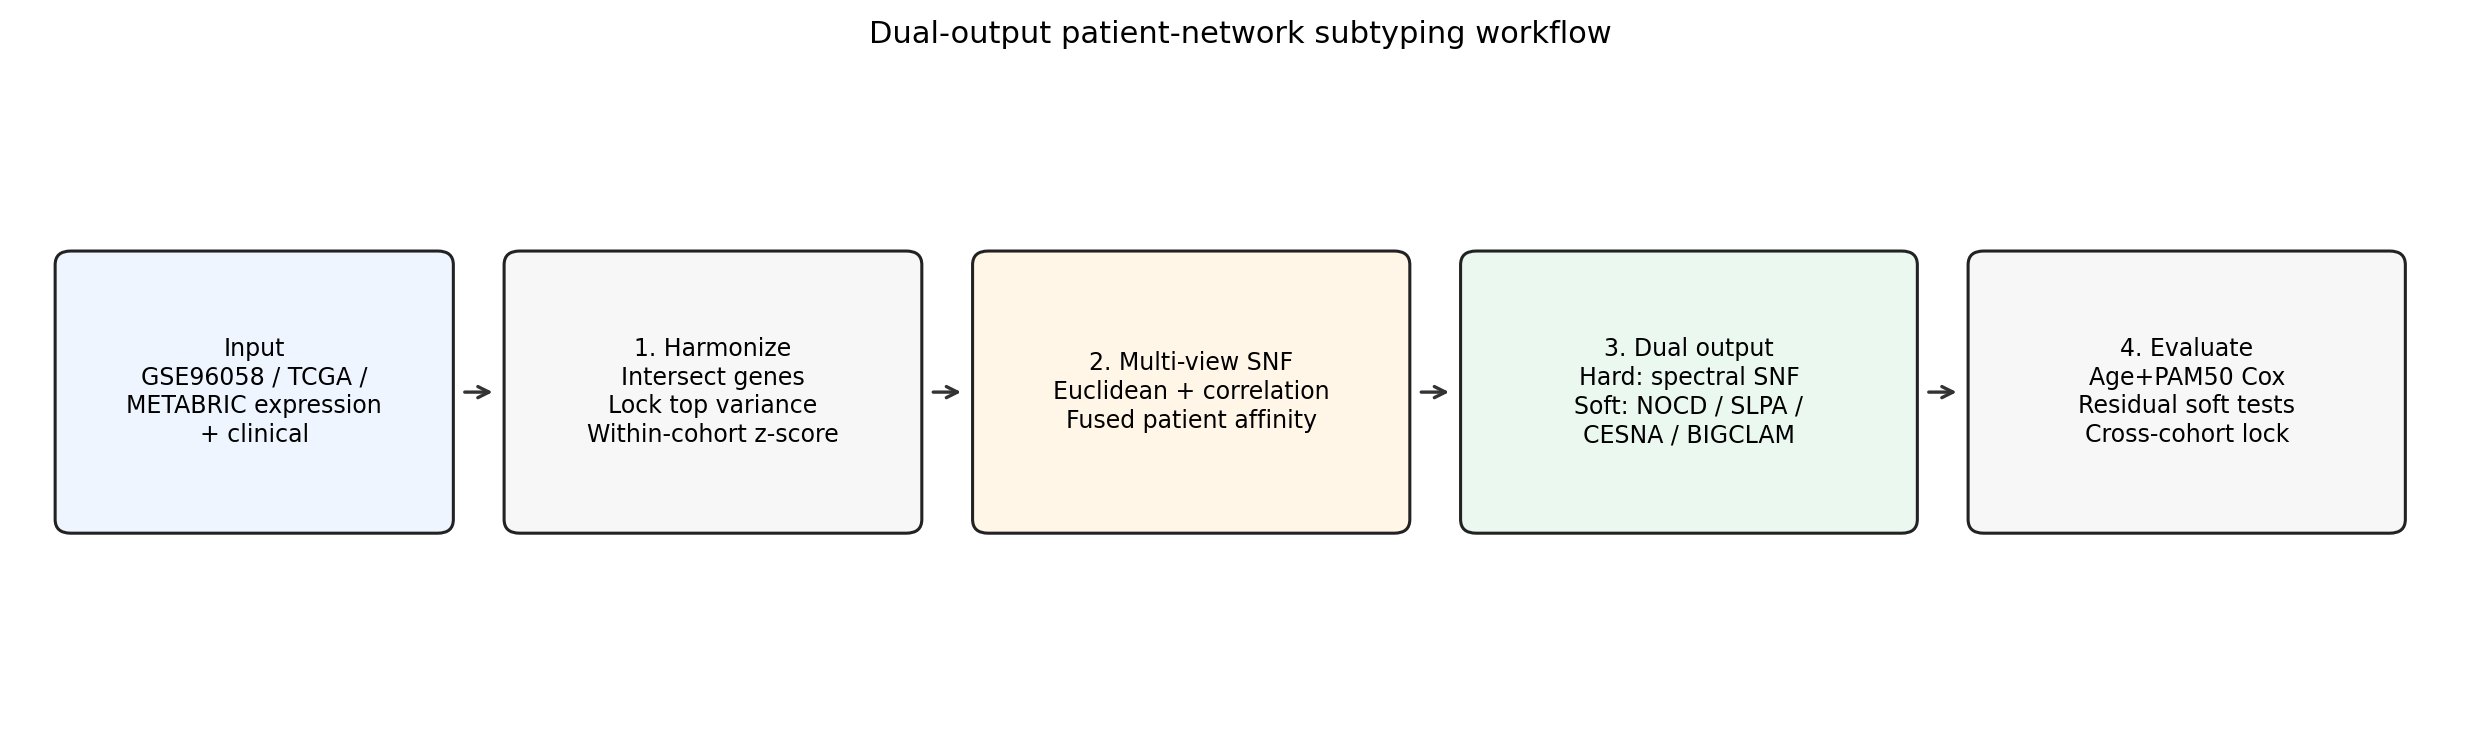
\includegraphics[width=\textwidth]{fig_pipeline.png}
\caption{Dual-output workflow. Multi-view SNF yields fused affinity and a hard spectral partition. The fused affinity is sparsified to a symmetric $k$NN graph (top-$15$ neighbours, symmetrized, components bridged). Overlapping engines are fit on that graph. Discovery locks are applied unchanged to validation cohorts.}
\label{fig:pipeline}
\end{figure}

\subsection{Harmonization and community-count lock}
Intersect gene symbols across cohorts. On \textbf{discovery only}, rank intersecting genes by variance and keep the top $2{,}000$. Apply that locked list to TCGA and METABRIC; z-score gene-wise \textbf{within each cohort}. Community count $K$ is locked on discovery by bootstrap stability: for each candidate $K\in\{4,\ldots,8\}$, labels are refit on bootstrap samples and mean pairwise adjusted Rand index (ARI) is recorded; we select $K=5$ (mean ARI $\approx 0.85$), the maximum in that grid (\texttt{results/q1/stability.csv}).

\subsection{Multi-view SNF and sparsification}
We implement classical SNF message-passing fusion~\cite{ref_snf} (Wang et al.\ iterative cross-diffusion; local $k$NN affinities, $T=15$ iterations, neighbourhood size $k=15$) on two views: Euclidean and Pearson-correlation distances converted to $k$NN affinities. Hard labels use scikit-learn spectral clustering on the fused affinity. The affinity argument is precomputed, and the assign-labels argument is kmeans, written \verb|assign_labels="kmeans"|. $K=5$ and the random seed is $42$. For soft engines, sparsify the fused affinity to a symmetric $k$NN adjacency ($k=15$) and reconnect components by bridging with the strongest fused similarities.

\subsection{Overlapping engines}
Soft $F\in\mathbb{R}^{n\times K}$ from: \textbf{NOCD-X} (expression-PCA node features) and \textbf{NOCD-G} (graph-derived features)---two-layer GCN, Bernoulli--Poisson loss, $250$ epochs~\cite{ref_nocd}; \textbf{SLPA} ($40$ iterations)~\cite{ref_slpa}; \textbf{CESNA-lite} (graph loss + linear reconstruction of expression PCs; CESNA-inspired~\cite{ref_cesna}); \textbf{BIGCLAM} classical affiliation~\cite{ref_bigclam} (baseline only). Mixed status: second/first affiliation ratio $\ge r$. On discovery, $r$ is chosen \emph{per engine} from $\{0.50,0.60,\ldots,0.95\}$ to place the mixed fraction nearest the centre of the usable window $[0.10,0.40]$ (engines that cannot enter the window keep the closest candidate). Locked values: NOCD-X $0.60$, NOCD-G $0.90$, SLPA $0.80$, CESNA-lite $0.70$, BIGCLAM $0.50$. Differences across engines therefore reflect scale/peakiness of each $F$, not arbitrary fixed cutoffs.

\subsection{Lead decision policy}
A~priori: BIGCLAM role $=\texttt{baseline\_comparison}$ (not lead-eligible). Quality filters on METABRIC: mixed fraction $\in[0.10,0.40]$; median peak ratio $<0.85$; LumA odds ratio $>1$. Lead $=$ sole lead-eligible engine in the quality-pass pool (ranked by hard Cox if several). No engine was excluded before fitting; failures are post-hoc filter fails. The lead designation reflects this pre-specified policy of reserving classical baselines for comparison; it is \textbf{not} a claim that NOCD-X outperforms BIGCLAM on every metric (BIGCLAM has stronger LumA OR and a nominal residual $p$).

\subsection{Evaluation}
Primary hard endpoint: Cox LR test of community indicators given age+PAM50~\cite{ref_cox}. We report uncorrected $p$ and Benjamini--Hochberg $q$ for the primary families~\cite{ref_bh}. The hard-method BH family is five methods. The METABRIC soft residual BH family is five engines. The GSE25066 BH family is two Fisher tests per engine. Soft: residual Cox (hard+mixed/entropy vs hard), PAM50 enrichment, programme scores for mixed vs single. Nested concordance (Harrell $C$)~\cite{ref_harrell}: point $\Delta C$ plus $200$-resample patient bootstrap $95\%$ CI for $\Delta C$ (age+PAM50 vs age+PAM50+SNF). Hard baselines also include Leiden~\cite{ref_leiden} and NMF~\cite{ref_nmf}. Soft bake-off metrics are \textbf{METABRIC-primary}; GSE96058/TCGA soft residuals are summarised for completeness. PAM50 hard labels are a reference taxonomy (unadjusted log-rank only).

\subsection{Ceiling experiments}
On the locked fused affinities we re-sparsify METABRIC at $k\in\{5,10,15,30\}$ and refit SLPA, BIGCLAM, and NOCD-X. This sweep uses a reduced budget ($80$ BIGCLAM iterations, one restart; $60$ NOCD epochs) and does not replace the locked bake-off. The same budget is used for an L1 grid, for Euclidean-only and correlation-only graphs, and for mixed-membership graphs ($n=300$) matched to the observed mean degrees. Biology uses the locked membership matrices: age-adjusted Cox of mixed and high-margin boundary flags inside each hard cluster and inside LumA; IntClust and Claudin-low odds ratios; within-cluster programme and locked-gene contrasts on METABRIC, repeated for programmes on SCAN-B. BH is applied inside each of those families. Hormone therapy and chemotherapy are modelled only if those columns are already on the harmonized clinical table.

\paragraph{GSE25066 response test.}
The locked $2{,}000$ symbols are intersected with GPL96. Where several probes map to one symbol, the probe with the highest variance is kept; that choice does not use pCR. Expression is z-scored within the cohort. SNF uses the same $k=15$, $T=15$, and spectral cut $K=5$ (\texttt{random\_state=42}). NOCD-X ($250$ epochs, expression features) and BIGCLAM ($250$ iterations, $5$ restarts, L1 $0.01$) are fit on the symmetrized $k$NN graph. Mixed status uses the locked ratios $0.60$ and $0.50$. The pre-stated primary family is two two-sided Fisher tests of pCR in mixed versus single patients: inside PAM50 LumA, and inside the hard cluster that contains the most mixed patients among clusters with at least $15$ mixed and $15$ single. BH is applied inside that pair. BIGCLAM is the same two tests in a separate family and cannot change the lead. As a sensitivity check that does not change the lock, the discovery SNF graph was rebuilt on the $1{,}400$ genes measured by the array, with the same $K$, $k$, $T$, and seed. Soft engines were not refit.

\section{Results}

\subsection{Hard SNF prognosis}
METABRIC age+PAM50 Cox: spectral SNF $p\approx 1.7\times10^{-4}$ (BH $q\approx 8.3\times10^{-4}$ within the five-method METABRIC family; Table~\ref{tab:hard}, Figure~\ref{fig:cox}). Single-view Euclidean and correlation spectral cuts are weaker on the adjusted endpoint ($p\approx 0.002$ and $0.010$). SNF+$k$-means on the fused affinity is competitive ($p\approx 8\times10^{-5}$); we retain spectral SNF as the pre-specified classical SNF hard cut and report $k$-means as a sensitivity analysis (Figure~\ref{fig:ablate}). Nested $C$-index point estimates: METABRIC $0.614\to 0.624$ ($\Delta C=0.011$); TCGA $0.666\to 0.687$ ($\Delta C=0.021$). Patient-bootstrap $95\%$ CIs for $\Delta C$ all \textbf{include zero} (METABRIC $[-0.007,0.010]$; TCGA $[-0.031,0.033]$; GSE96058 $[-0.009,0.007]$; $n_{\mathrm{boot}}\approx 200$), all within bootstrap noise, and are not claimed as statistically or clinically decisive. KM curves with risk tables and log-rank $p$ are in Figure~\ref{fig:km_snf}.

\begin{table}[htbp]
\centering
\caption{Hard partitions: age+PAM50 Cox $p$ / BH $q$ (METABRIC $q$ within five-method family).}
\label{tab:hard}
\begin{tabular}{lcccc}
\toprule
Method & GSE96058 $p$ & TCGA $p$ & METABRIC $p$ & METABRIC $q$ \\
\midrule
SNF (primary) & $0.062$ & $0.073$ & $\mathbf{1.7\times10^{-4}}$ & $\mathbf{8.3\times10^{-4}}$ \\
Leiden & $0.275$ & $0.132$ & $0.003$ & $0.008$ \\
NMF & $0.030$ & $0.212$ & $0.010$ & $0.017$ \\
BIGCLAM hard (baseline) & $0.166$ & $0.217$ & $0.022$ & $0.028$ \\
Consensus & $0.220$ & $0.055$ & $0.077$ & $0.077$ \\
\bottomrule
\end{tabular}
\end{table}

\begin{figure}[H]
\centering
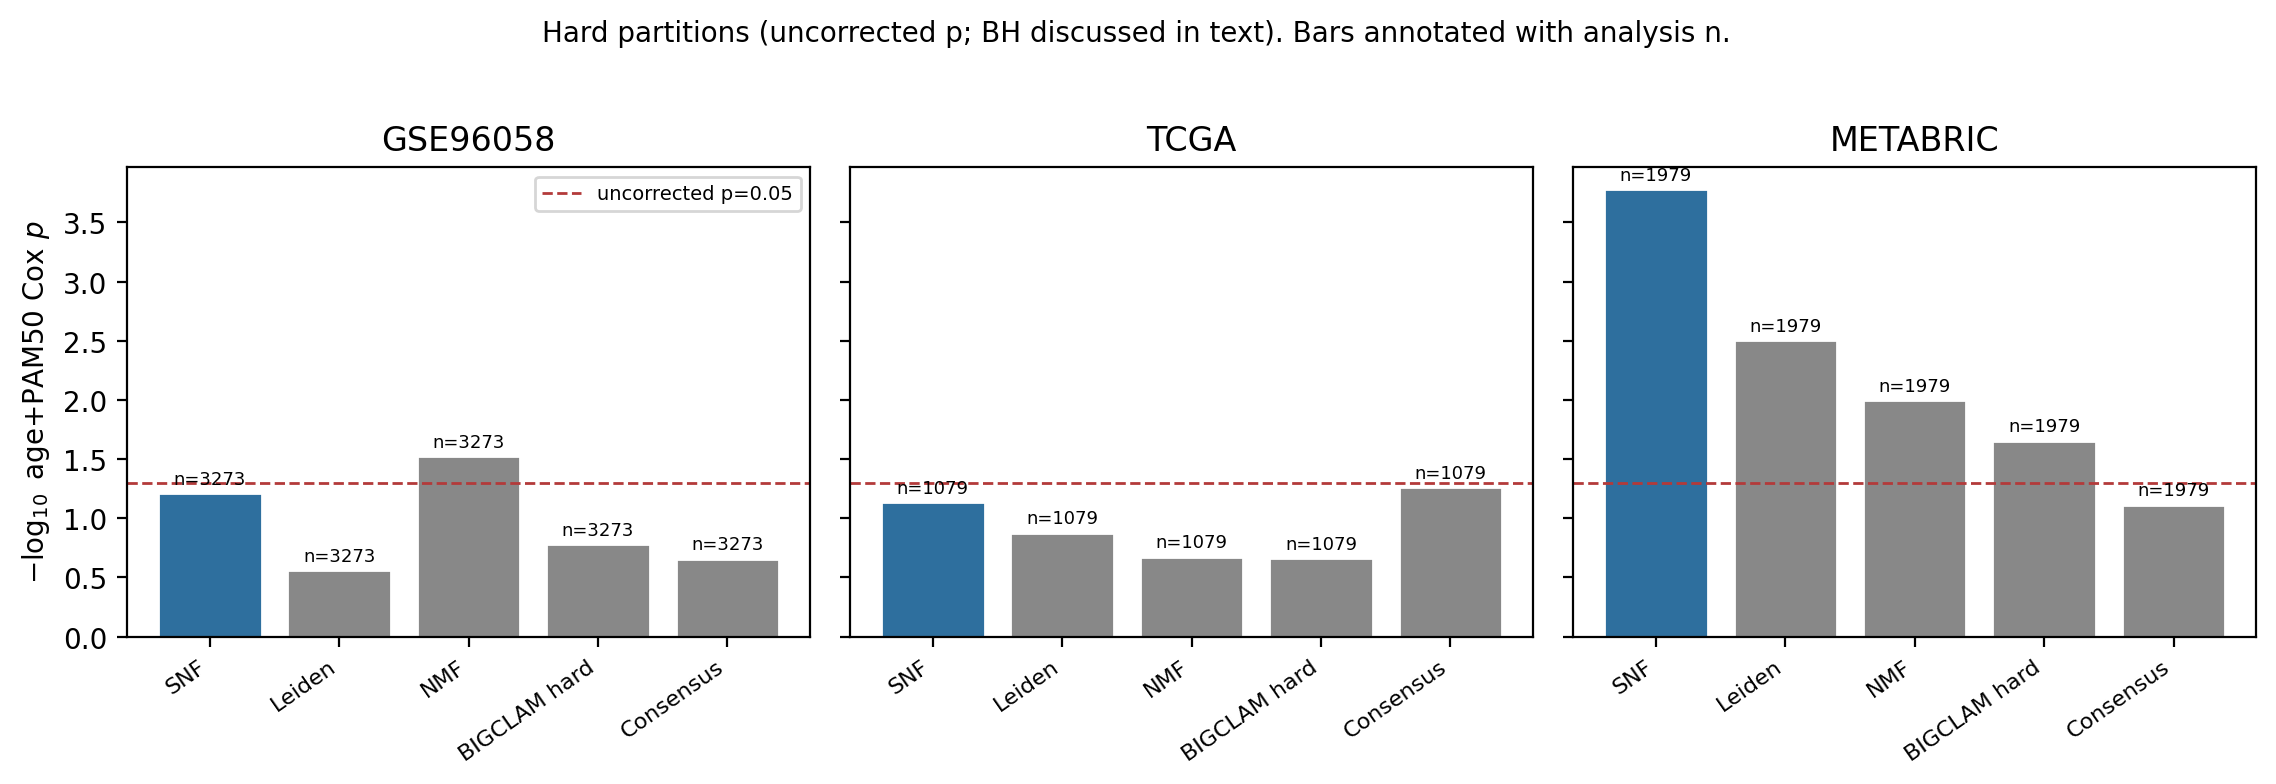
\includegraphics[width=\textwidth]{fig_cox_bars.png}
\caption{Age+PAM50 Cox strength ($-\log_{10}p$, uncorrected) with analysis $n$ on each bar. Dashed line: uncorrected $p=0.05$.}
\label{fig:cox}
\end{figure}

\begin{figure}[H]
\centering
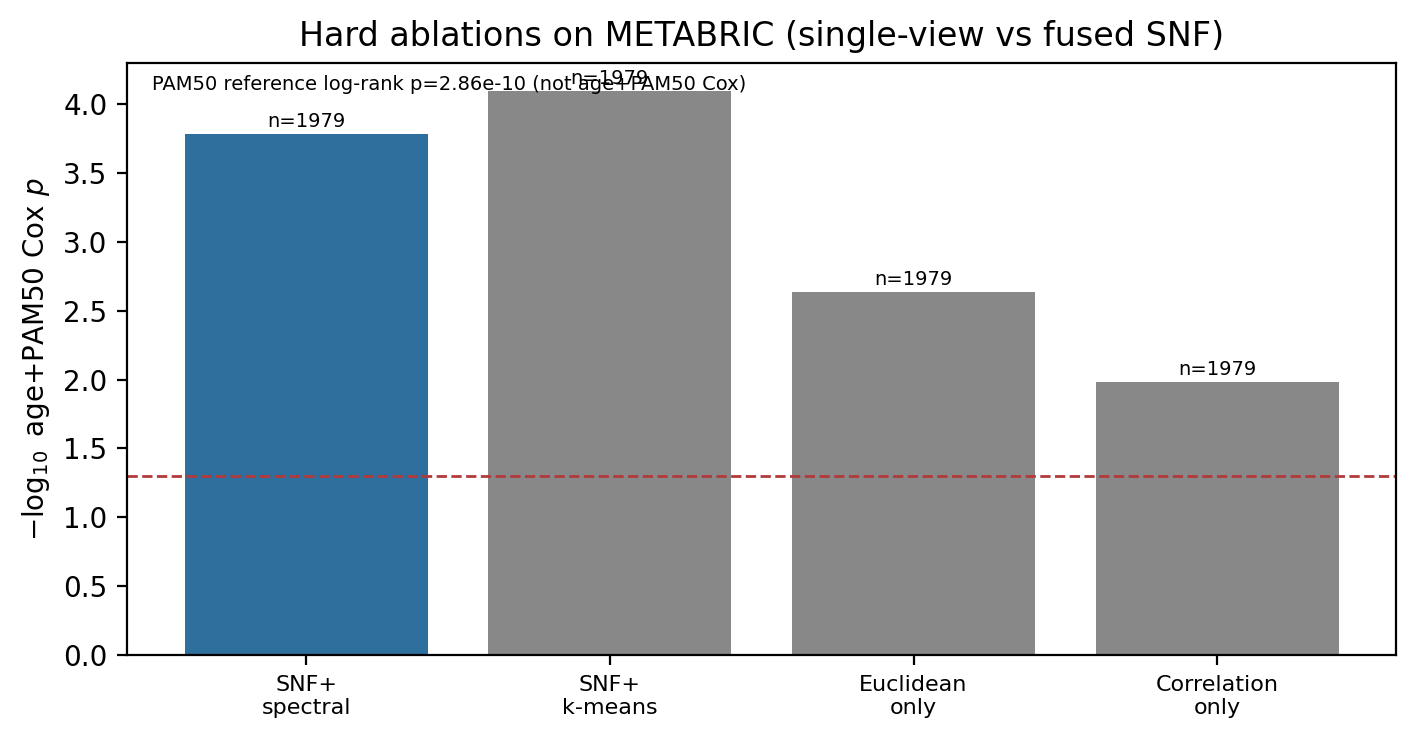
\includegraphics[width=0.85\textwidth]{fig_hard_ablations.png}
\caption{METABRIC hard ablations: fused SNF vs single-view spectral cuts (age+PAM50 Cox).}
\label{fig:ablate}
\end{figure}

\begin{figure}[htbp]
\centering
\begin{subfigure}{0.32\textwidth}
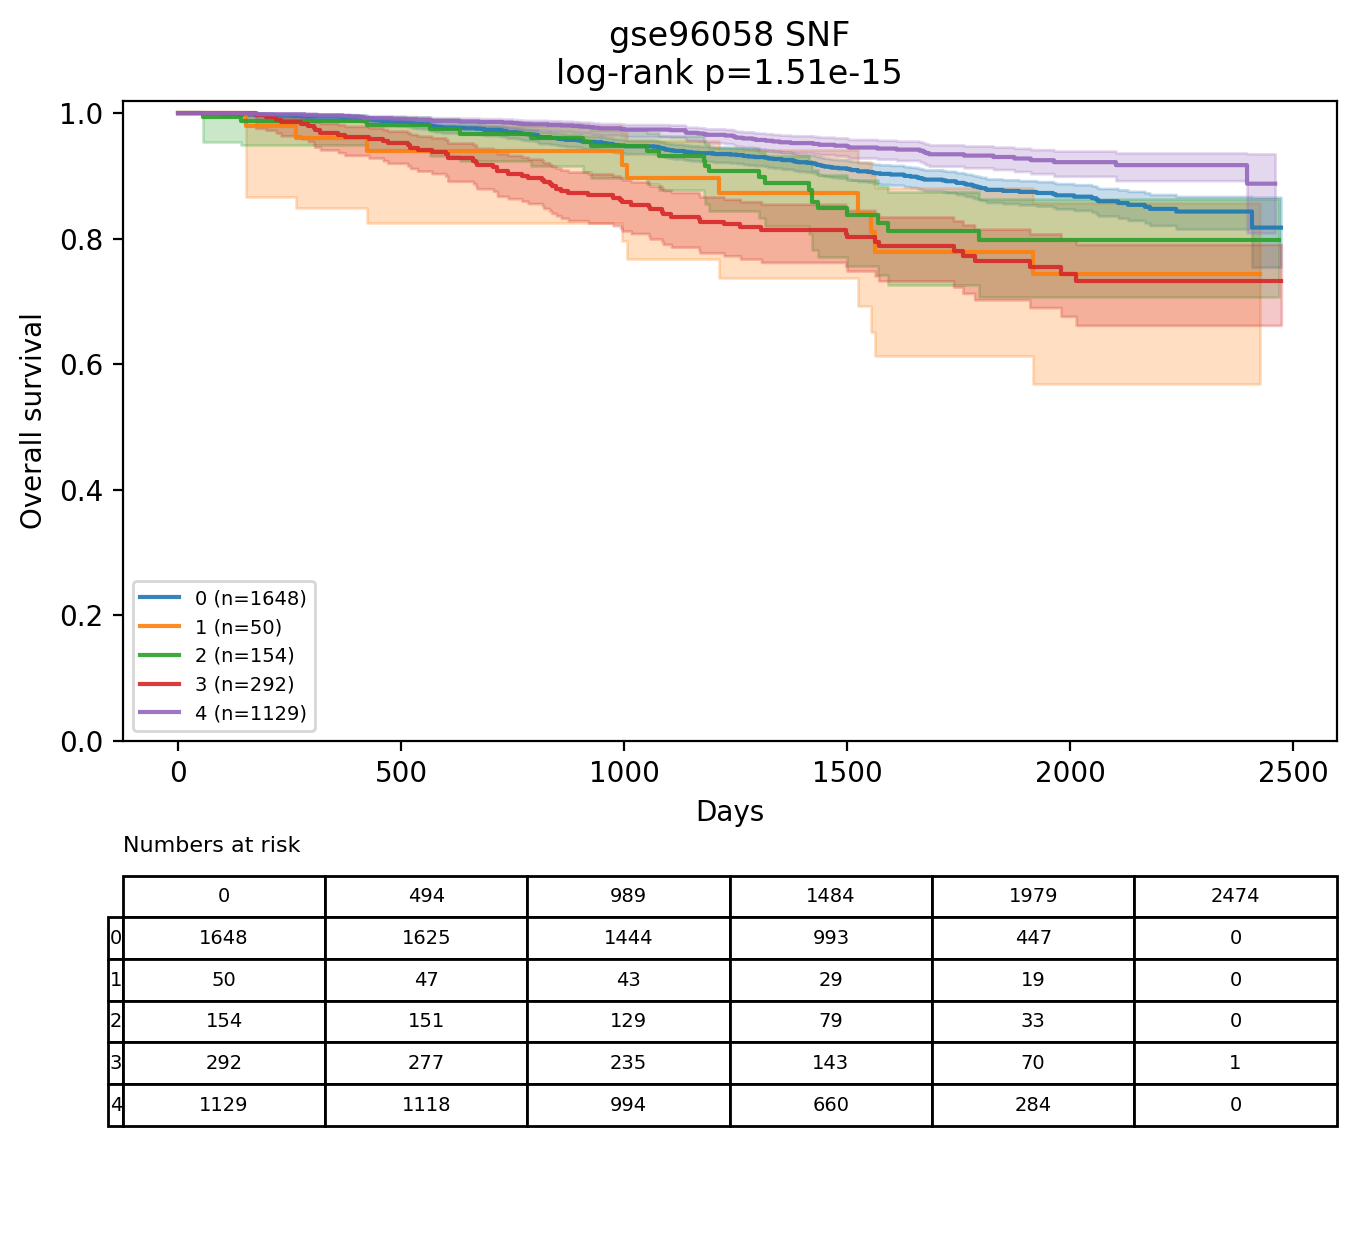
\includegraphics[width=\linewidth]{fig_km_snf_gse.png}
\caption{GSE96058}
\end{subfigure}\hfill
\begin{subfigure}{0.32\textwidth}
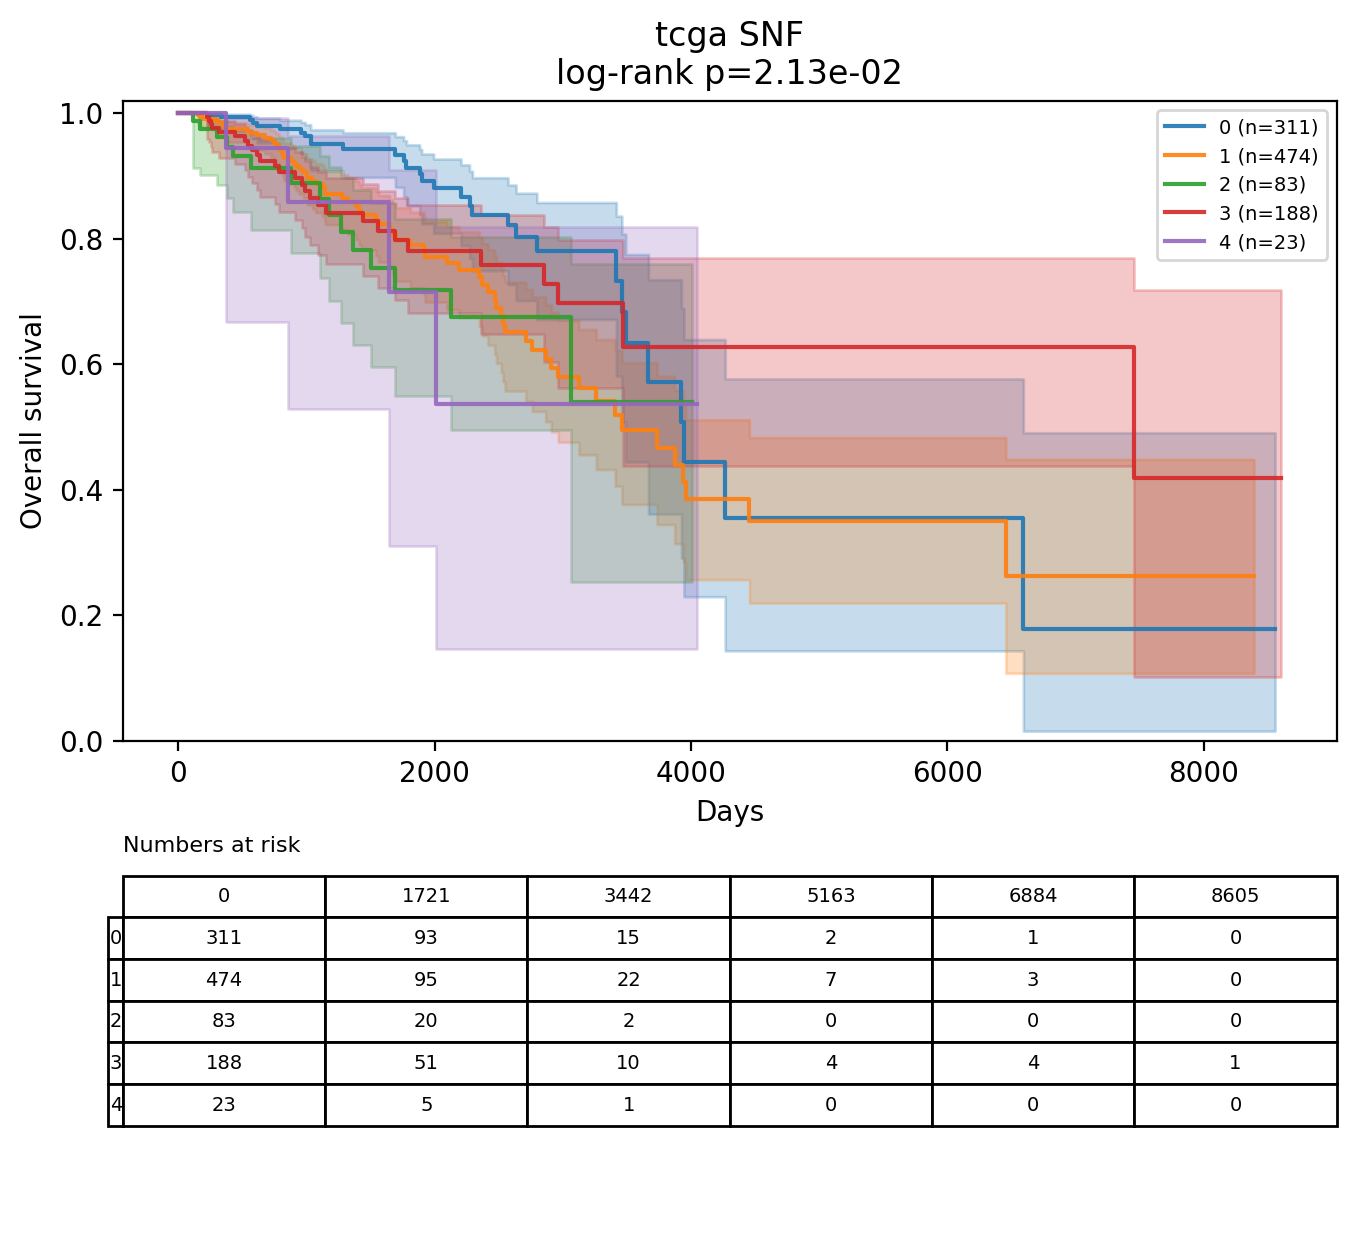
\includegraphics[width=\linewidth]{fig_km_snf_tcga.png}
\caption{TCGA}
\end{subfigure}\hfill
\begin{subfigure}{0.32\textwidth}
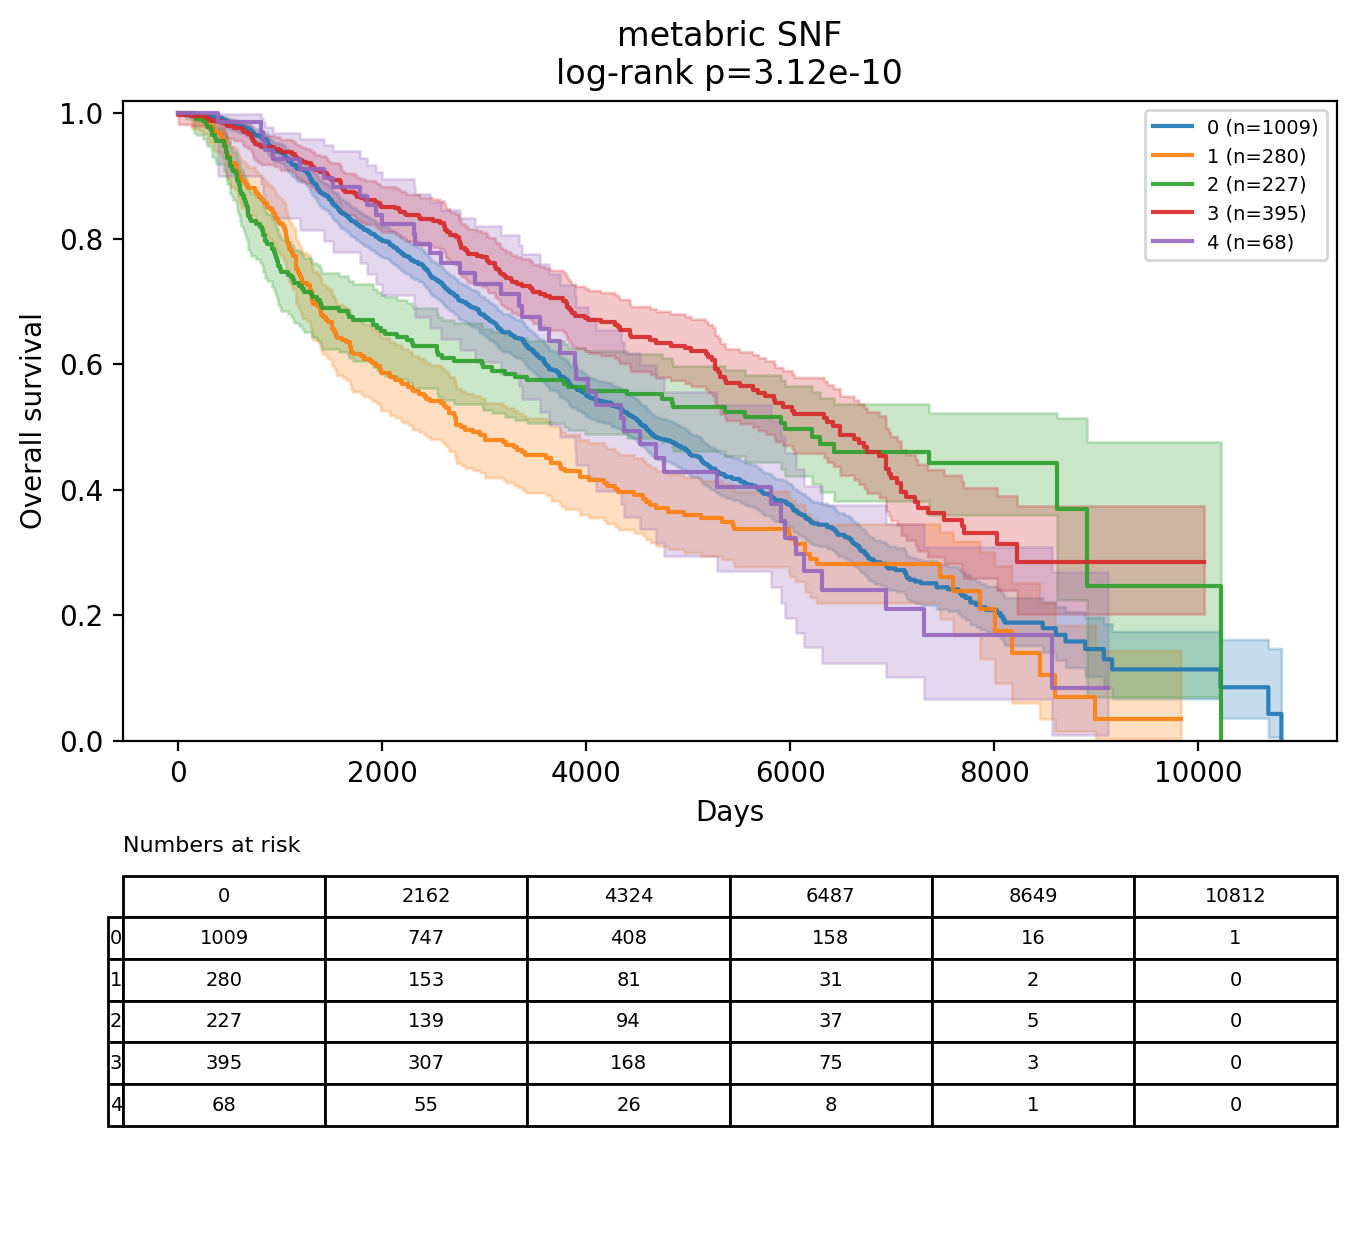
\includegraphics[width=\linewidth]{fig_km_snf_metabric.png}
\caption{METABRIC}
\end{subfigure}
\caption{Hard SNF Kaplan--Meier curves with numbers at risk. (a)~GSE96058, (b)~TCGA-BRCA, (c)~METABRIC.}
\label{fig:km_snf}
\end{figure}

\subsection{Soft lead decision (METABRIC-primary)}
Soft residual bake-off and quality filters are \textbf{METABRIC-primary} (longest follow-up / most events). GSE96058 and TCGA own-hard+mixed residuals are reported for completeness and are mostly null after BH within cohort. The exception, also for completeness, is SLPA on TCGA ($p\approx 0.004$, $q\approx 0.022$), which still fails the quality filters (\texttt{tables/soft\_cross\_cohort\_summary.csv}).

Table~\ref{tab:decision} / Figure~\ref{fig:decision} show every engine against every filter. BIGCLAM \textbf{passes} all quality filters but is \textbf{not lead-eligible} by the a~priori baseline policy. Among eligible engines, only NOCD-X passes all three filters and is therefore the soft lead. This is a policy choice, not a claim that NOCD-X dominates BIGCLAM on LumA enrichment or residual $p$. SLPA yields the smallest METABRIC residual $p$ ($0.0055$; BH $q\approx 0.028$) but fails every quality filter: mixed fraction $\approx 69\%$, median peak ratio $=1$ (second affiliation equals the first for typical patients), and LumA depletion. That peak ratio stays $1$ after sparsification (Section~\ref{sec:closed}), so the collapse is not a $k$NN setting left untuned. The residual test then revisits a near-consensus partition and is not read as a usable soft phenotype.

BIGCLAM's residual own-hard+mixed signal ($p\approx 0.036$) yields BH $q\approx 0.091$ across the five-engine METABRIC soft family and therefore \textbf{fails FDR at the $0.05$ threshold}; we state the uncorrected $p$ for transparency but do not treat it as multiplicity-robust evidence.

\begin{table}[htbp]
\centering
\caption{Lead decision (METABRIC). Pass/fail per criterion. BIGCLAM passes the quality filters and remains ineligible for the lead.}
\label{tab:decision}
\resizebox{\textwidth}{!}{%
\begin{tabular}{lccccccc}
\toprule
Method & Role & Mixed 10--40\% & Peak $<0.85$ & LumA OR$>1$ & Quality & Eligible & Lead \\
\midrule
SLPA & candidate & Fail & Fail & Fail & Fail & Yes & No \\
BIGCLAM & baseline & Pass & Pass & Pass & Pass & No & No \\
CESNA-lite & candidate & Pass & Pass & Fail & Fail & Yes & No \\
NOCD-G & candidate & Pass & Pass & Fail & Fail & Yes & No \\
NOCD-X & candidate & Pass & Pass & Pass & Pass & Yes & Yes \\
\bottomrule
\end{tabular}}
\end{table}

\begin{figure}[htbp]
\centering
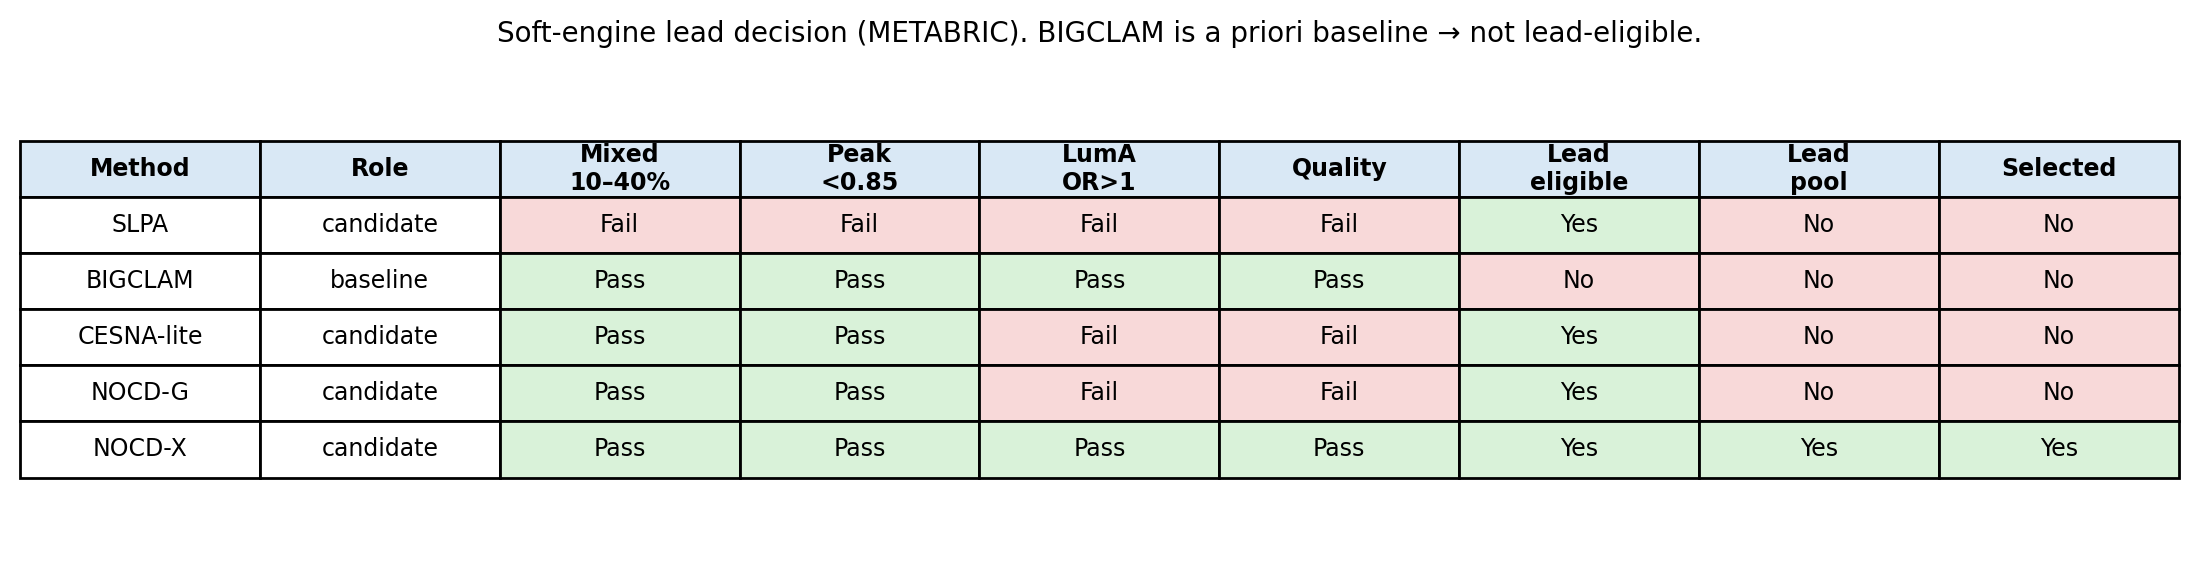
\includegraphics[width=\textwidth]{fig_lead_decision.png}
\caption{Explicit pass/fail lead decision. BIGCLAM quality-pass but baseline-ineligible.}
\label{fig:decision}
\end{figure}

\begin{figure}[htbp]
\centering
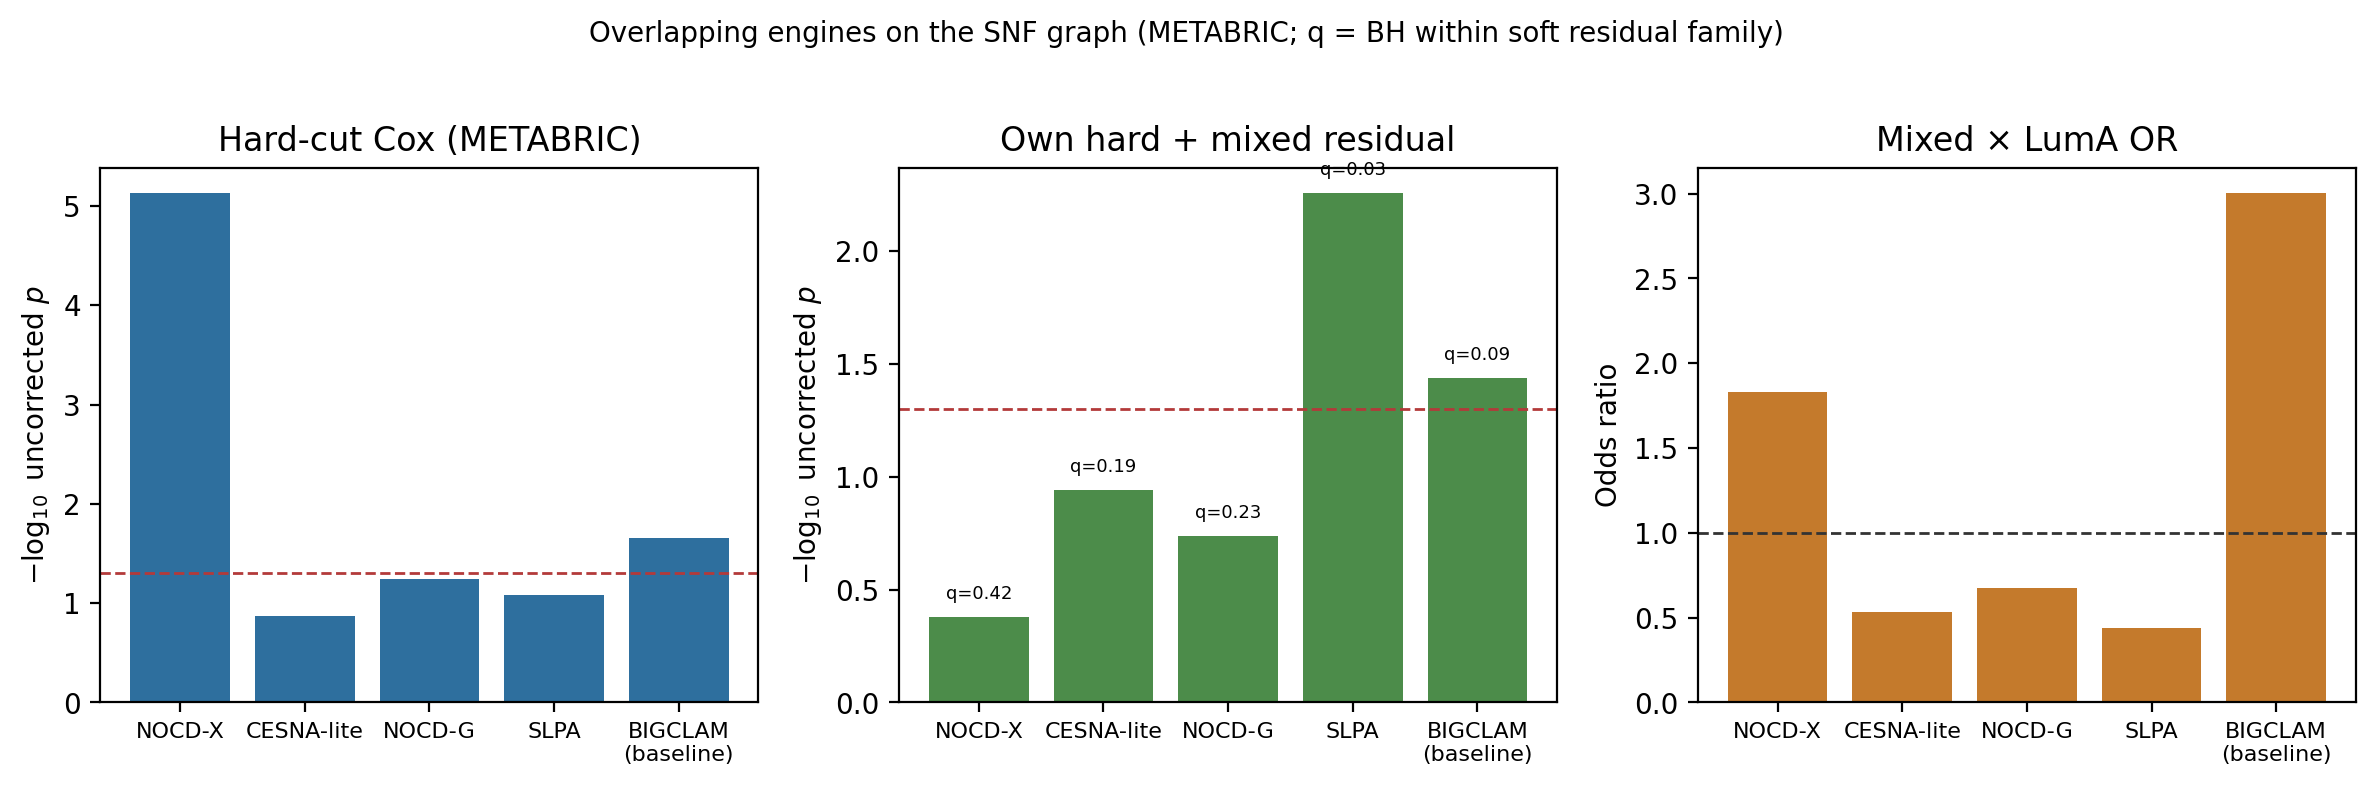
\includegraphics[width=\textwidth]{fig_soft_bakeoff.png}
\caption{Soft bake-off on METABRIC. Left: $-\log_{10}$ \emph{uncorrected} hard-cut Cox $p$. Middle: $-\log_{10}$ \emph{uncorrected} own-hard+mixed residual $p$, with BH $q$ annotated for the family of five METABRIC soft engines. Right: LumA odds ratios.}
\label{fig:soft}
\end{figure}

\subsection{Biology of mixed membership}
Mixed patients are LumA-enriched under NOCD-X and BIGCLAM (Figure~\ref{fig:enrich}), not Claudin-low. Programme scores (Figure~\ref{fig:programs}; positive $=$ higher in mixed): mixed tumours show higher estrogen-programme and lower basal/proliferation mean $z$-scores (BIGCLAM estrogen $\Delta\approx +0.56$ SD units, $n_{\mathrm{mixed}}=504$, $p\approx 6\times10^{-42}$; NOCD-X $\Delta\approx +0.36$ SD, $n_{\mathrm{mixed}}=334$, $p\approx 3\times10^{-9}$). These are moderate standardised shifts ($\sim 0.4$--$0.6$ within-cohort SD), made highly significant by large $n$; we interpret them as a coherent luminal-leaning mixed phenotype rather than a large clinical effect size per se. Top gene contrasts are in \texttt{tables/mixed\_top\_genes.csv}.

\begin{figure}[htbp]
\centering
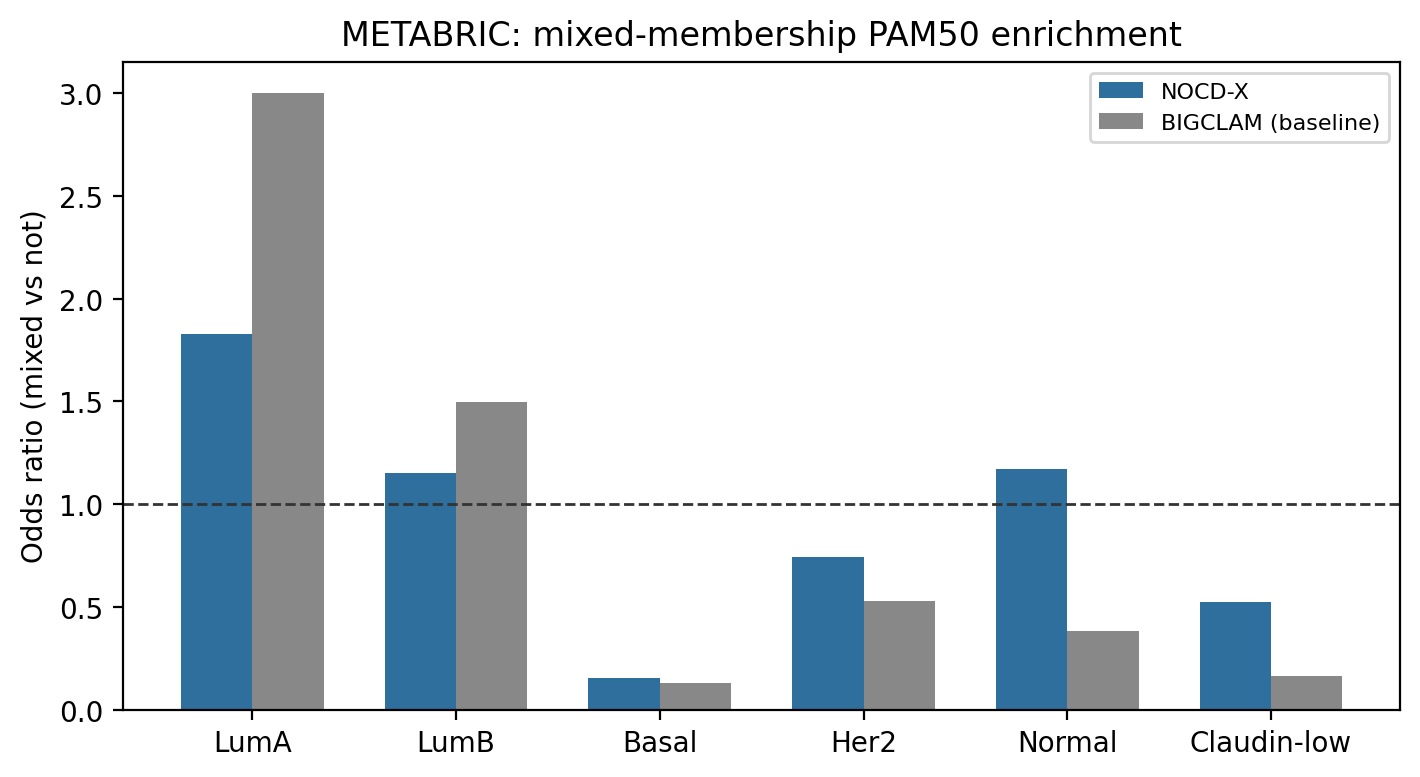
\includegraphics[width=0.75\textwidth]{fig_mixed_enrichment.png}
\caption{METABRIC mixed$\times$PAM50 odds ratios (NOCD-X vs BIGCLAM baseline).}
\label{fig:enrich}
\end{figure}

\begin{figure}[htbp]
\centering
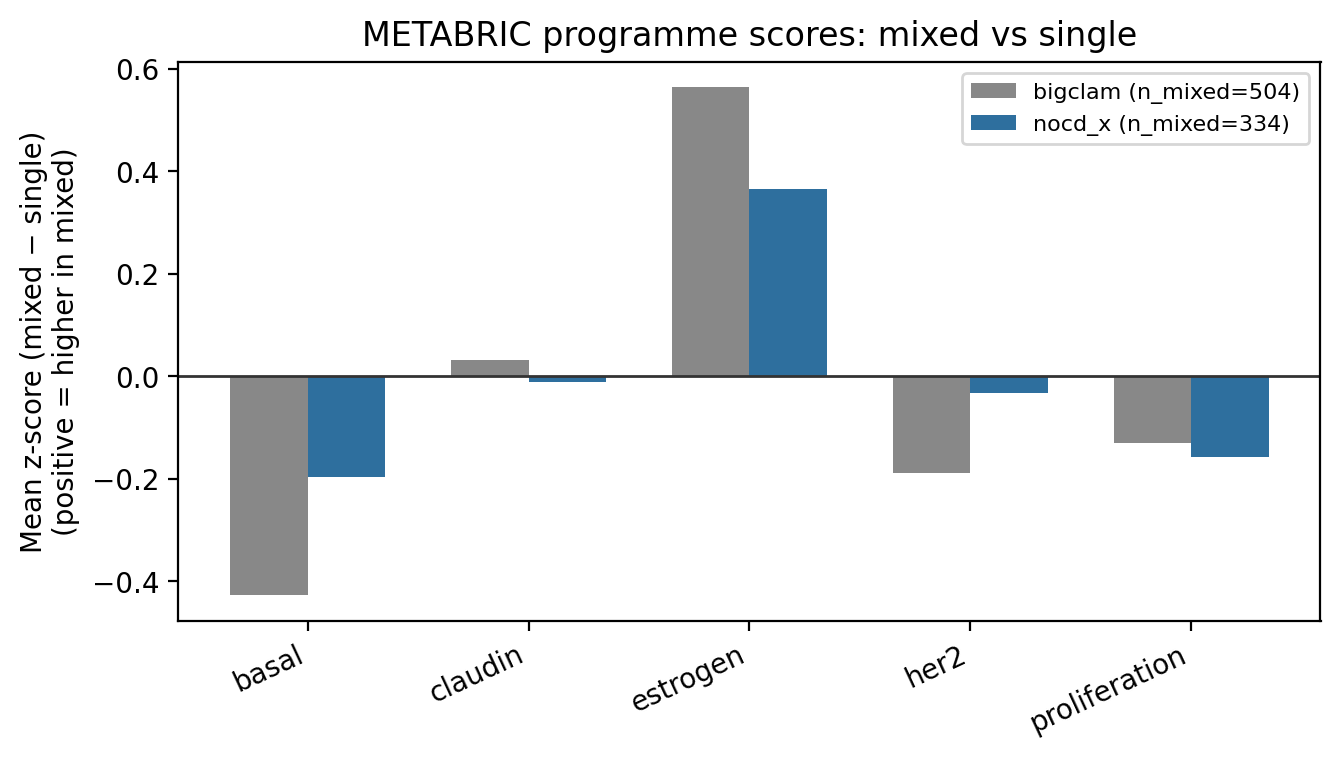
\includegraphics[width=0.72\textwidth]{fig_mixed_programs.png}
\caption{METABRIC curated programme scores. $y$-axis: mean $z$-score (mixed $-$ single); positive means higher in mixed. Sample sizes in the legend ($n_{\mathrm{mixed}}$).}
\label{fig:programs}
\end{figure}

\begin{figure}[htbp]
\centering
\begin{subfigure}{0.48\textwidth}
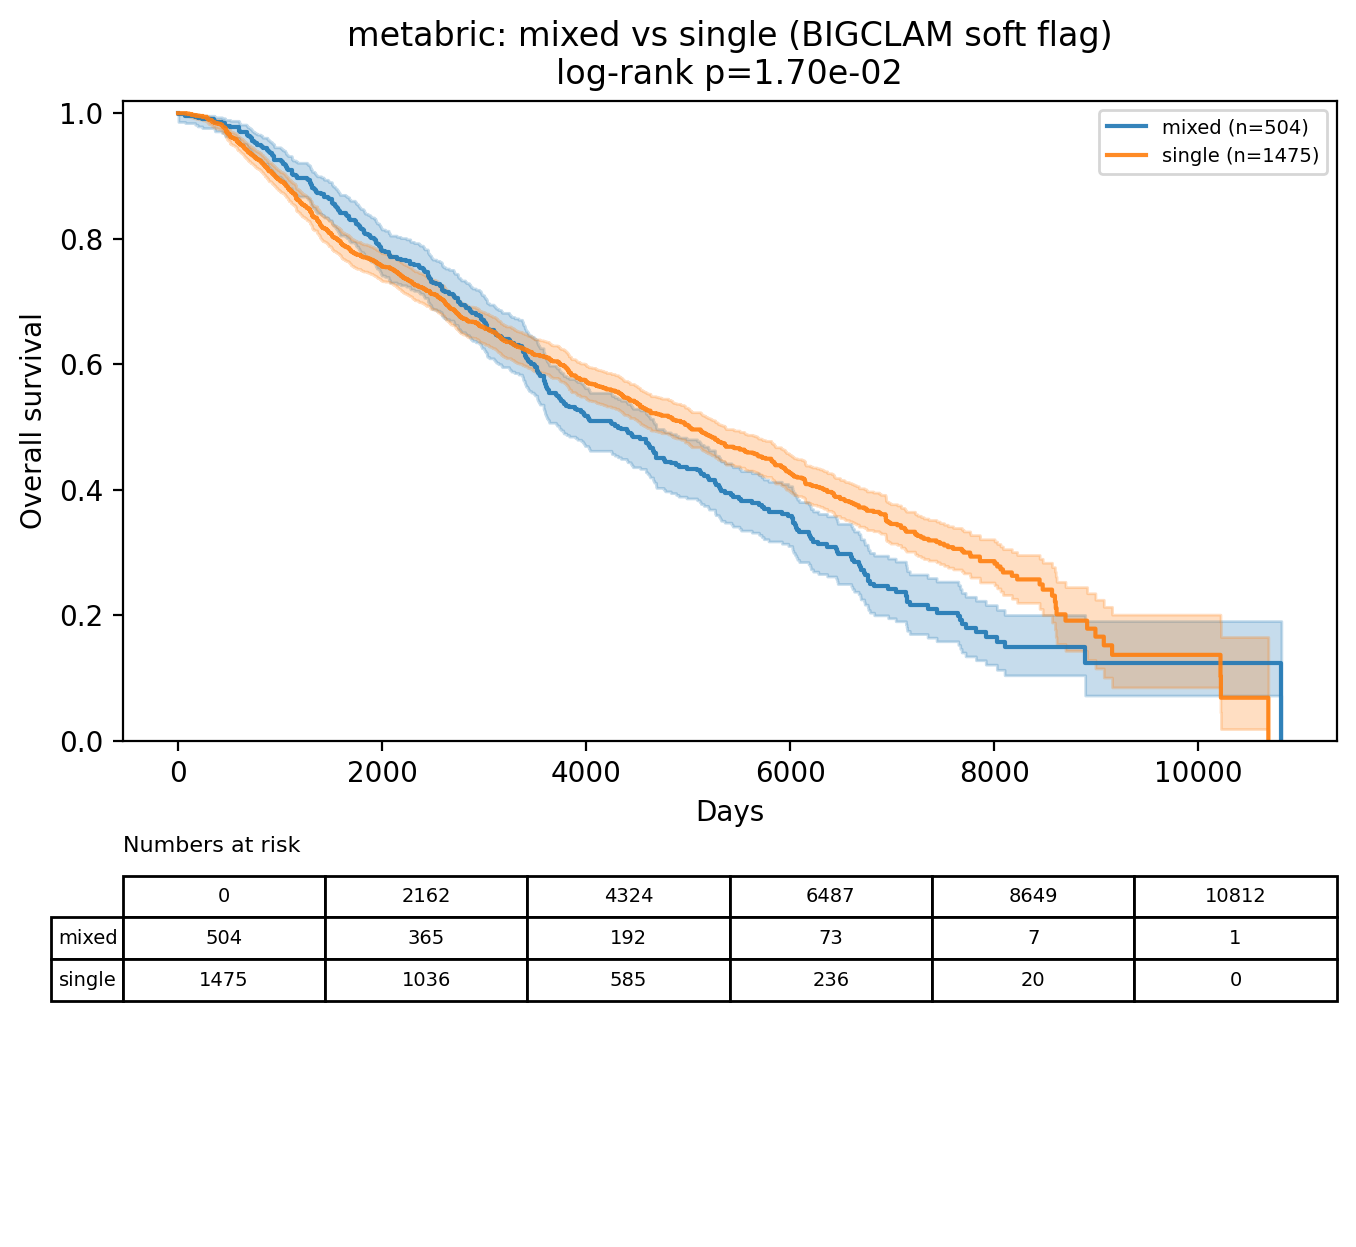
\includegraphics[width=\linewidth]{fig_km_mixed_metabric.png}
\caption{Mixed vs single}
\end{subfigure}\hfill
\begin{subfigure}{0.48\textwidth}
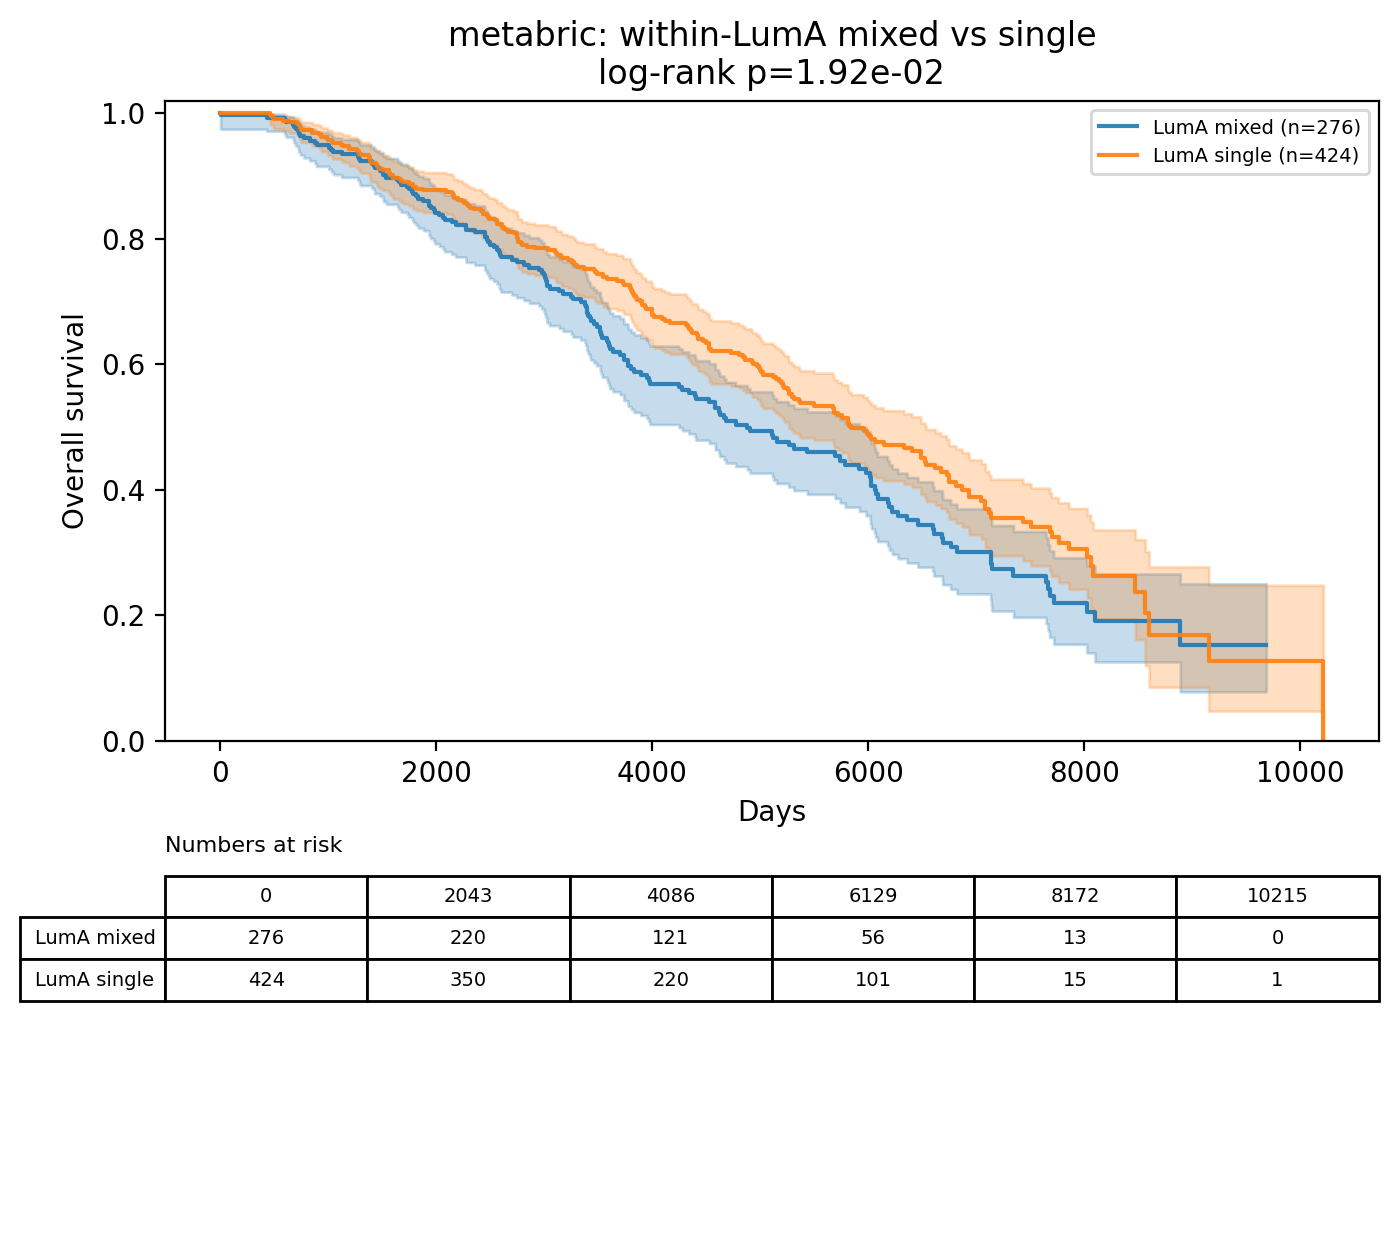
\includegraphics[width=\linewidth]{fig_km_within_luma_metabric.png}
\caption{Within LumA}
\end{subfigure}
\caption{METABRIC Kaplan--Meier curves for the BIGCLAM mixed flag, with numbers at risk. (a)~mixed versus single, (b)~the same contrast inside LumA.}
\label{fig:km_soft}
\end{figure}

\subsection{Closed routes}
\label{sec:closed}
Checks that could have supported a stronger claim are negative. They are reported as nulls.

\paragraph{SLPA is not rescued by sparsification.}
On the locked METABRIC fused affinity, $k\in\{5,10,15,30\}$ spans mean degree $6.4$ to $34$. SLPA's median second/first affiliation is $1.0$ at every value (mixed fraction $0.83$, $0.77$, $0.69$, $0.51$; Figure~\ref{fig:density}). Within this range the collapse is a property of SLPA on the fused affinity, not an obvious under-sparsification.

\paragraph{No prognostic subgroup inside the hard cut.}
Age-adjusted Cox tests of mixed and high-margin boundary flags, inside each hard cluster and inside LumA, do not survive BH. The smallest METABRIC $q$ is $0.23$. There is no clinical-refinement claim.

\paragraph{L1 does not explain BIGCLAM versus NOCD-X.}
BIGCLAM L1 in $\{0,10^{-3},10^{-2},10^{-1}\}$ leaves LumA OR at $3.00$ and residual $p$ at $0.56$. The gap between BIGCLAM's LumA OR ($\approx 3.0$, locked residual $q \approx 0.091$) and NOCD-X's weaker OR is not an L1 artifact on this grid.

The fourth check, pathological complete response, is reported separately (Section~\ref{sec:pcr}).

\begin{figure}[H]
\centering
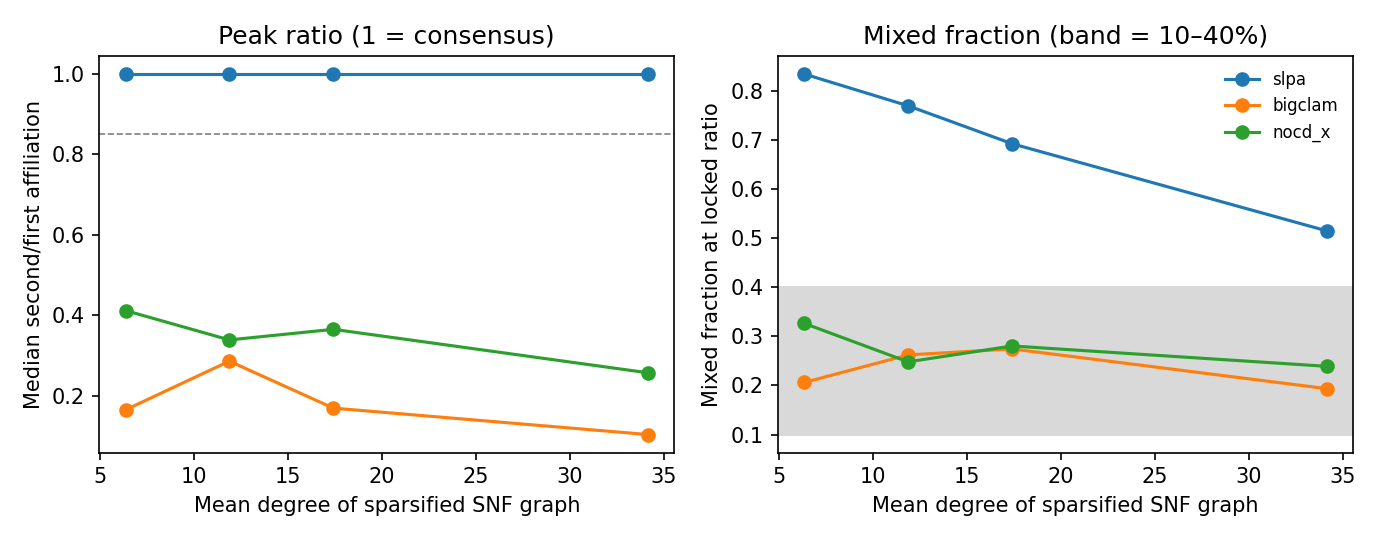
\includegraphics[width=\textwidth]{fig_density_sweep.png}
\caption{METABRIC density sweep on the locked fused affinity. Left: median second/first affiliation (dashed line $0.85$). Right: mixed fraction at the locked ratio; the band is $10$--$40\%$. SLPA stays at peak ratio $1$ across the degree range.}
\label{fig:density}
\end{figure}

\subsection{Treatment-response test}
\label{sec:pcr}
GSE25066~\cite{ref_hatzis} asks whether mixed patients have a lower pathological complete response under the locked pipeline. The pre-stated primary family is two two-sided Fisher tests for NOCD-X (mixed ratio $0.60$): inside PAM50 LumA, and inside the hard cluster with the most mixed patients. BH is applied inside that pair. BIGCLAM (mixed ratio $0.50$) is the same two tests in a separate family and is not lead-eligible. The soft membership is not associated with pCR in GSE25066 under locked settings (Table~\ref{tab:pcr}). Rebuilding the discovery graph on the $1{,}400$ shared genes leaves the hard partition close to the locked one (ARI $0.89$) and the fused affinities highly correlated (Spearman $0.98$), so the locked settings are kept for GSE25066. Soft engines were not refit. Details are in the Discussion.

\begin{table}[htbp]
\centering
\caption{GSE25066 pCR, mixed versus single. Families are BH-adjusted separately. BIGCLAM cannot become the lead. The asterisk marks an odds ratio of 0: the BIGCLAM mixed group inside LumA had zero pCR events. The Fisher $p$ is the reported test.}
\label{tab:pcr}
\begin{tabular}{llrrrrr}
\toprule
Engine & Scope & pCR mixed & pCR single & OR & $p$ & BH $q$ \\
\midrule
\multicolumn{7}{l}{\emph{Primary family: NOCD-X}} \\
NOCD-X & LumA & 1/35 & 4/118 & 0.84 & 1.00 & 1 \\
NOCD-X & Hard cluster 1 & 2/34 & 14/134 & 0.54 & 0.53 & 1 \\
\midrule
\multicolumn{7}{l}{\emph{Baseline family: BIGCLAM, not lead-eligible}} \\
BIGCLAM & LumA & 0/29 & 5/124 & $0^{\ast}$ & 0.58 & 1 \\
BIGCLAM & Hard cluster 1 & 3/30 & 13/138 & 1.07 & 1.00 & 1 \\
\bottomrule
\end{tabular}
\end{table}

The LumA stratum has five pCR events. The hard-cluster stratum has sixteen pCR events. The LumA contrast is event-poor, and the hard-cluster contrast is better powered and still null. There is no treatment-resistance claim.

\subsection{Checks that do not override the policy}
Two remaining levers were run before the framing above. Neither makes NOCD-X the better estimator, so neither is used to defend the lead.

On mixed-membership graphs matched to these mean degrees ($n=300$), mean correlation with the true soft membership is $0.53$ for BIGCLAM, $0.17$ for SLPA, and $0.10$ for graph-feature NOCD. Mixed-label ARI is below $0.10$ for every engine. Ground truth, at this budget, agrees with the direction of the LumA odds ratio: the classical baseline recovers more of the planted membership. That is why the lead is not reassigned. Reassigning it to BIGCLAM would violate the pre-specified rule; reassigning the narrative so that NOCD-X ``wins on truth'' would contradict the simulation.

IntClust is an orthogonal label, and the soft flag does track it (Figure~\ref{fig:intclust}). NOCD-X mixed patients are depleted in IntClust~10 (OR $0.058$, $q=2.4\times10^{-14}$) and Claudin-low (OR $0.53$, $q=0.013$) and enriched in IntClust~7 (OR $1.95$, $q=0.0014$). BIGCLAM is enriched more strongly in IntClust~8 (OR $3.24$, $q=5.3\times10^{-18}$), and also in IntClust~7 and~3, with Claudin-low OR $0.16$. Inside BIGCLAM hard cluster 0 the programme shifts are small (estrogen $\Delta=+0.088$ SD, $n_{\mathrm{mixed}}=410$; HER2 $\Delta=-0.185$; proliferation $\Delta=-0.129$). SCAN-B repeats estrogen-up and HER2-down for BIGCLAM inside hard cluster 0 (estrogen $\Delta=+0.081$ SD; HER2 $\Delta=-0.514$; proliferation $\Delta=+0.165$, the opposite direction; \texttt{results/ceiling/program\_contrasts.csv}). This is external agreement with a luminal-versus-basal axis, stronger for the baseline than for the policy lead. It is not a new subtype and not a reason to change the lead. A reduced-budget view ablation uses the same fit as the density sweep ($80$ BIGCLAM iterations and one restart; $60$ NOCD epochs) on the Euclidean, correlation, and fused graphs (\texttt{results/ceiling/view\_ablation.csv}). It does not replace the locked bake-off. On that ablation the LumA enrichment is specific to the fused graph: BIGCLAM's LumA OR is $3.00$ (fused), $1.35$ (Euclidean), and $0.91$ (correlation). NOCD-X LumA ORs on the same fits are $0.97$ (fused), $0.86$ (Euclidean), and $0.86$ (correlation).

\begin{figure}[H]
\centering
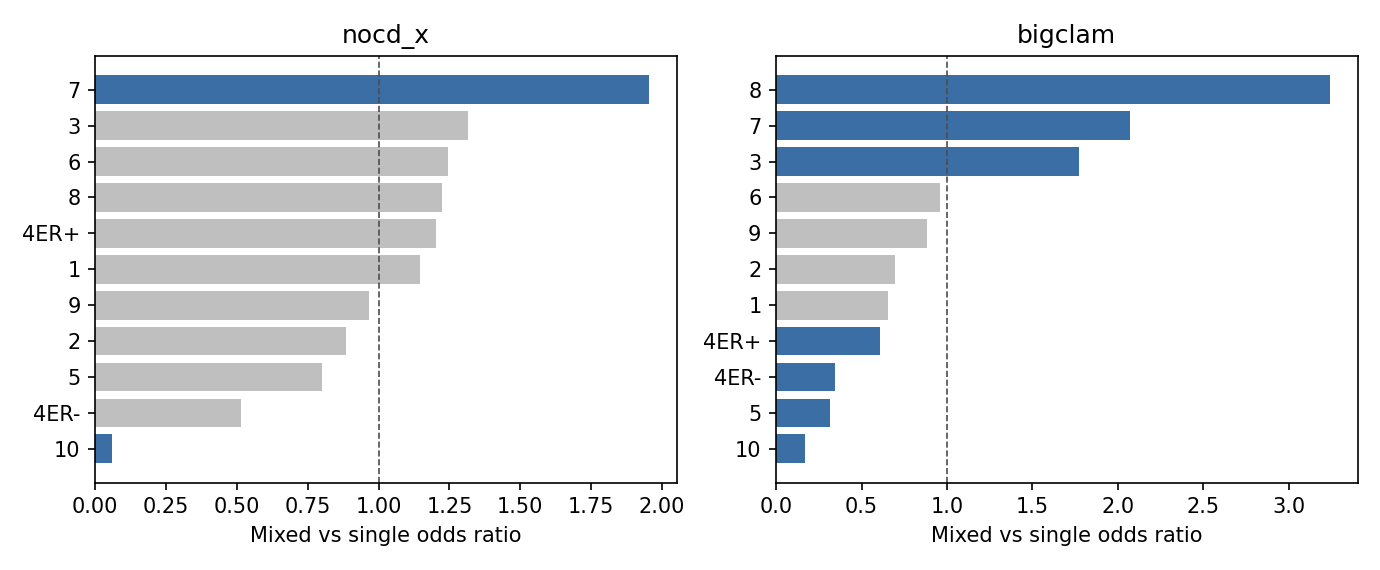
\includegraphics[width=\textwidth]{fig_intclust_or.png}
\caption{METABRIC mixed-versus-single odds ratios by IntClust. Blue bars have BH $q<0.05$ inside that engine's orthogonal-label family.}
\label{fig:intclust}
\end{figure}

\section{Discussion}

The result this study can defend is methodological. A locked protocol and a pre-specified baseline rule keep a stronger LumA odds ratio, a stronger IntClust enrichment, and a higher simulation correlation from being rewritten as the lead method. BIGCLAM shows those point estimates and still fails FDR on the residual test ($q \approx 0.091$). The simulation and IntClust benchmarks favor BIGCLAM on point estimates, which is why the policy, not the metric, determines the lead. NOCD-X is the lead because it is the only eligible engine inside the quality-pass pool, not because it dominates BIGCLAM.

The routes that would have raised the claim are null. SLPA collapse survives sparsification down to mean degree $6$, with mixed fractions rising from $0.51$ to $0.83$ as $k$ falls from $30$ to $5$. Boundary survival inside hard clusters and inside LumA does not survive BH (smallest METABRIC $q \approx 0.23$). L1 does not explain the LumA odds-ratio gap. The nested concordance gain, $\Delta C$, has a $95\%$ CI that includes zero on every cohort.

GSE25066 was run under the locked settings and was null. Mixed status is not associated with pathological complete response. The LumA stratum has five pCR events (NOCD-X $1/35$ versus $4/118$; OR $0.84$; $p=1.00$). Hard cluster 1, the cluster with the most mixed patients, has sixteen pCR events (NOCD-X $2/34$ versus $14/134$; OR $0.54$; $p=0.53$). The LumA contrast is event-poor. The hard-cluster contrast is better powered and is still null (BH $q=1$ inside the pre-stated two-test family). BIGCLAM, in a separate family, is not lead-eligible and is also null. Age, stage, grade, residual cancer burden, and distant relapse-free survival are stored in \texttt{results/gse25066/assignments.csv} and were not used as covariates. No hormone-therapy or chemotherapy column was added to SCAN-B, TCGA, or METABRIC. The null does not validate the soft membership.

The GSE25066 graph is built on $1{,}400$ of $2{,}000$ locked genes ($70\%$). Rebuilding the discovery graph on those $1{,}400$ genes leaves the hard partition close to the locked one (ARI $0.89$) and the fused affinities highly correlated (Spearman $0.98$). Soft engines were not refit, and the gene list was not changed. Other limits: expression-only fusion; the simulation and the L1 grid use a shorter fit than the locked bake-off ($80$ BIGCLAM iterations and one restart, and $60$ NOCD epochs, against $250$ iterations with five restarts and $250$ epochs); programme tests use the locked $2{,}000$ genes rather than the $1{,}400$ shared with GSE25066, so the programme scores are not directly comparable across the discovery and treatment-response cohorts.

\section{Conclusion}
The hard SNF partition remains the positive result (METABRIC age+PAM50 Cox $p \approx 1.7\times10^{-4}$; BH $q \approx 8.3\times10^{-4}$ within five hard methods). Under locked settings, the GSE25066 treatment-response test is null in LumA (five pCR events) and in the hard cluster with the most mixed patients (sixteen pCR events). No treatment-resistance claim is made. NOCD-X remains the soft lead by the pre-specified rule, and the lead is not reversed.

\section{Data and code availability}
Public cohorts under their access terms. Code repository: \url{https://github.com/saeedsamimi995/snf-overlap-evaluation}. Tables: \texttt{lead\_decision\_table.csv}, \texttt{hard\_cox\_bh.csv} (Cox proportional-hazards BH), \texttt{soft\_residual\_bh.csv}, \texttt{delta\_c\_bootstrap.csv}, \texttt{soft\_cross\_cohort\_summary.csv}. Code: \texttt{run\_snf\_overlap\_sota.py}, \texttt{run\_snf\_bigclam\_study.py}, \texttt{python -m scripts.run\_ceiling\_experiments}, \texttt{python -m src.analysis.gse25066\_response}. Ceiling tables are in \texttt{results/ceiling/}, including \texttt{view\_ablation.csv} and \texttt{program\_contrasts.csv}. GSE25066 outputs are \texttt{results/gse25066/pcr\_tests.csv} and \texttt{results/gse25066/assignments.csv}. The assignment file contains age, ER/PR/HER2, stage, grade, pCR/RD, residual cancer burden, distant relapse-free survival, and PAM50. Only pCR, PAM50, and the hard SNF cluster entered the tests. Gene-overlap sensitivity is \texttt{results/gse25066/gene\_overlap\_sensitivity.json}. The identity call is \texttt{results/ceiling/decision\_note.md}. Environment: \texttt{environment.yml}.

\begin{thebibliography}{99}

\bibitem{ref_perou}
Perou CM, et al. Molecular portraits of human breast tumours. \textit{Nature}. 2000;406:747--752.

\bibitem{ref_sorlie}
S{\o}rlie T, et al. Gene expression patterns of breast carcinomas distinguish tumor subclasses with clinical implications. \textit{Proc Natl Acad Sci USA}. 2001;98:10869--10874.

\bibitem{ref_pam50}
Parker JS, et al. Supervised risk predictor of breast cancer based on intrinsic subtypes. \textit{J Clin Oncol}. 2009;27:1160--1167.

\bibitem{ref_metabric}
Curtis C, et al. The genomic and transcriptomic architecture of 2,000 breast tumours reveals novel subgroups. \textit{Nature}. 2012;486:346--352.

\bibitem{ref_intclust}
Dawson SJ, Rueda OM, Aparicio S, Caldas C. A new genome-driven integrated classification of breast cancer and its implications. \textit{EMBO J}. 2013;32:617--628.

\bibitem{ref_tcga}
The Cancer Genome Atlas Network. Comprehensive molecular portraits of human breast tumours. \textit{Nature}. 2012;490:61--70.

\bibitem{ref_tcga_pancan}
Hoadley KA, et al. Cell-of-origin patterns dominate the molecular classification of 10,000 tumors from 33 types of cancer. \textit{Cell}. 2018;173:291--304.e6.

\bibitem{ref_cbioportal}
Cerami E, et al. The cBio cancer genomics portal: an open platform for exploring multidimensional cancer genomics data. \textit{Cancer Discov}. 2012;2:401--404.

\bibitem{ref_scanb}
Brueffer C, et al. Clinical value of RNA sequencing--based classifiers for prediction of the five conventional breast cancer biomarkers: a report from the population-based multicenter SCAN-B study. \textit{JCO Precis Oncol}. 2018;2:1--18.

\bibitem{ref_saal}
Saal LH, et al. The Sweden Cancerome Analysis Network -- Breast (SCAN-B) Initiative: a large-scale multicenter infrastructure towards implementation of breast cancer genomic analyses in the clinical routine. \textit{Genome Med}. 2015;7:20. (GSE96058).

\bibitem{ref_snf}
Wang B, et al. Similarity network fusion for aggregating data types on a genomic scale. \textit{Nat Methods}. 2014;11:333--337.

\bibitem{ref_cancer_subtypes}
Xu T, et al. CancerSubtypes: an R/Bioconductor package for molecular cancer subtype identification, validation and visualization. \textit{Bioinformatics}. 2017;33:3131--3133.

\bibitem{ref_absnf}
Ruan P, et al. Using association signal annotations to boost similarity network fusion. \textit{Bioinformatics}. 2019;35:3718--3726.

\bibitem{ref_wsnf}
Xu T, Le TD, Liu L, Wang R, Sun B, Li J. Identifying cancer subtypes from miRNA-TF-mRNA regulatory networks and expression data. \textit{PLoS One}. 2016;11:e0152792.

\bibitem{ref_misssnf}
Gliozzo J, Soto Gomez MA, Bonometti A, Patak A, Casiraghi E, Valentini G. miss-SNF: a multimodal patient similarity network integration approach to handle completely missing data sources. \textit{Bioinformatics}. 2025;41:btaf150.

\bibitem{ref_nemo}
Rappoport N, Shamir R. NEighborhood-based Multi-Omics clustering (NEMO). \textit{Bioinformatics}. 2019;35:3059--3065.

\bibitem{ref_icluf}
Shakyawar SK, Sajja BR, Patel JC, Guda C. iCluF: an unsupervised iterative cluster-fusion method for patient stratification using multiomics data. \textit{Bioinform Adv}. 2024;4:vbae015. doi:10.1093/bioadv/vbae015.

\bibitem{ref_bigclam}
Yang J, Leskovec J. Overlapping community detection at scale: a nonnegative matrix factorization approach. In: \textit{Proceedings of the Sixth ACM International Conference on Web Search and Data Mining (WSDM)}. 2013:587--596.

\bibitem{ref_cesna}
Yang J, McAuley J, Leskovec J. Community detection in networks with node attributes. In: \textit{IEEE International Conference on Data Mining (ICDM)}. 2013:1151--1156.

\bibitem{ref_slpa}
Xie J, Szymanski BK, Liu X. SLPA: uncovering overlapping communities in social networks via a speaker-listener interaction dynamic process. In: \textit{2011 IEEE 11th International Conference on Data Mining Workshops (ICDMW)}. 2011:344--349. doi:10.1109/ICDMW.2011.154.

\bibitem{ref_nocd}
Shchur O, G\"unnemann S. Overlapping community detection with graph neural networks. In: \textit{Deep Learning on Graphs Workshop (DLG@KDD)}. 2019. arXiv:1909.12201.

\bibitem{ref_mmsb}
Airoldi EM, Blei DM, Fienberg SE, Xing EP. Mixed membership stochastic blockmodels. \textit{J Mach Learn Res}. 2008;9:1981--2014.

\bibitem{ref_fuzzy_hier}
Ciaramella A, Nardone D, Staiano A. Data integration by fuzzy similarity-based hierarchical clustering. \textit{BMC Bioinformatics}. 2020;21(Suppl 10):350. doi:10.1186/s12859-020-03567-6.

\bibitem{ref_ssmf}
Liu W, Murphy TB, Brennan L. Simplex-structured matrix factorisation: application of soft clustering to metabolomic data. \textit{Sci Rep}. 2025;15:17817. doi:10.1038/s41598-025-02361-9.

\bibitem{ref_leiden}
Traag VA, Waltman L, van Eck NJ. From Louvain to Leiden: guaranteeing well-connected communities. \textit{Sci Rep}. 2019;9:5233. doi:10.1038/s41598-019-41695-z.

\bibitem{ref_nmf}
Lee DD, Seung HS. Learning the parts of objects by non-negative matrix factorization. \textit{Nature}. 1999;401:788--791.

\bibitem{ref_cox}
Cox DR. Regression models and life-tables. \textit{J R Stat Soc Series B}. 1972;34:187--220. doi:10.1111/j.2517-6161.1972.tb00899.x.

\bibitem{ref_harrell}
Harrell FE Jr, et al. Evaluating the yield of medical tests. \textit{JAMA}. 1982;247:2543--2546.

\bibitem{ref_bh}
Benjamini Y, Hochberg Y. Controlling the false discovery rate: a practical and powerful approach to multiple testing. \textit{J R Stat Soc Series B}. 1995;57:289--300. doi:10.1111/j.2517-6161.1995.tb02031.x.

\bibitem{ref_hatzis}
Hatzis C, et al. A genomic predictor of response and survival following taxane-anthracycline chemotherapy for invasive breast cancer. \textit{JAMA}. 2011;305:1873--1881.

\end{thebibliography}

\end{document}
